\documentclass[10pt,a4paper]{article}
\usepackage[utf8]{inputenc}
\usepackage[czech]{babel}
\usepackage[T1]{fontenc}
\usepackage{amsmath}
\usepackage{amsfonts}
\usepackage{amssymb}
\usepackage{graphicx}
\usepackage{float}
\author{Martin Žid}
\title{4. Seznámení se se zvolenou pokročilou iterativní metodou na problému batohu}
\date{}
\begin{document}

\maketitle

\section{Zadání}
\begin{itemize}
 \item Zvolte si heuristiku, kterou budete řešit problém vážené splnitelnosti booleovské formule (simulované ochlazování, simulovaná evoluce, tabu prohledávání).
 \item Tuto heuristiku použijte pro řešení problému batohu. Můžete použít dostupné instance problému, anebo si vygenerujte své instance pomocí generátoru. Používejte instance s větším počtem věcí (>30).
 \item Hlavním cílem domácí práce je seznámit se s danou heuristikou, zejména se způsobem, jakým se nastavují její parametry (rozvrh ochlazování, selekční tlak, tabu lhůta…) a modifikace (zjištění počáteční teploty, mechanismus selekce, tabu atributy...).
\end{itemize} 

 \subsection{Zpráva by měla obsahovat} 
  \begin{itemize}
   \item Stručný popis zvoleného algoritmu.
   \item Zhodnocení Vašich experimentů. Zkoušejte sledovat vývoj řešení (populace u GA) v průběhu běhu algoritmu.
   \item Experimentujte s různými nastaveními parametrů.
   \item Výsledek měření = čas výpočtu a rel. chyba. Pokud nejste schopni vypočítat rel. chybu, stačí uvést vývoj výsledné ceny (počáteční -- koncová).
   \item Pokuste se vyvodit nějaké závěry.
  \end{itemize}
  
\section{Rozbor možných variant řešení}
V této úloze jsme měli možnost výběru jedné ze tří pokročilých iterativních technik.
Algoritmy k výběru:
\begin{itemize}
 \item simulované ochlazování,
 \item genetické algoritmy,
 \item tabu search.
\end{itemize}
Pro řešení této úlohy jsem si zvolil metodu simulovaného ochlazování.

\section{Rámcový popis postupu řešení}
V první části jsem se seznámil s metodou simulovaného ochlazování. Po implementaci této pokročilé iterativní techniky byly výsledky otestovány s exaktními řešeními. Následně probíhalo měření relativní chyby a počtu navštívených stavů v závislosti na jednotlivých parametrech algoritmu. Při měření byl měněn vždy pouze jeden parametr a ostatní byly zafixovány.

\section{Popis kostry algoritmu}
Algoritmus má nastavitelné čtyři parametry: počáteční teplotu, koncovou teplotu, $equilibrium$ a koeficient ochlazování.

Na začátku je vybrán počáteční stav, což je implementováno jako prázdný batoh a teplota je rovna počáteční teplotě. Následný výpočet probíhá ve dvou cyklech. Počet iterací vnějšího cyklu udává funkce $frozen$ a vnitřního cyklu funkce $equilibrium$. Funkce $frozen$ vrací $true$, pokud teplota dosáhla hodnoty koncové teploty. Funkce $equilibrium$ vrací $true$, pokud je počet iterací na dané teplotě menší než $n * equilibrium$.

Ve vnitřním cyklu je volána funkce $try$. Funkce $try$ náhodně zvolí (změnou jednoho bitu vektoru konfigurace) souseda aktuálního stavu. Pokud je tento soused lepší než daný stav, pak je vrácen. Pokud není, je vrácen pouze pokud $ x < e^{\frac{-\delta}{teplota}}$. Kde x je náhodné číslo z intervalu 0, 1 a $\delta$ je rozdíl cen nového a aktuálního stavu. Ve všech ostatních případech je vrácen původní stav.

Ve vnitřním cyklu je ještě testováno zda nemá aktuální stav lepší cenu než nejlepší naleznou. Pokud ano, pak je daný stav uložen jako nejlepší.

Po doběhnutí vnitřního cyklu $equilibria$ je volá funkce $cool$, která vynásobí teplotu koeficientem ochlazování. Tento koeficient je v rozmezí 0,8 až 0,99 (teplotu tedy zmenší).

\section{Naměřené výsledky}
Základní nastavení algoritmu bylo: počáteční teplota = 100, koeficient ochlazování = 0,9, teplota tuhnutí = 10, $equilibrium$ = 5. Chyba simulovaného ochlazovaní byla počítána pomocí vzorce pro relativní chybu $\epsilon = \frac{C(opt) - C(apx)}{C(opt)}$. Chyba i počet navštívených stavů byly měřeny vždy pro celý soubor, tedy padesát problému, kde výsledky byly následně zprůměrovány.

\begin{table}[H]
\centering
  \begin{tabular}{ |c|c|c|}
  \hline
  Počáteční teplota & Relativní chyba & Počet stavů \\
  \hline
  30  & 0,0281 & 110000 \\
  50  & 0,0151 & 160000 \\
  100 & 0,0107 & 220000 \\ 
  150 & 0,0105 & 260000 \\
  200 & 0,0098 & 290000 \\
  300 & 0,0105 & 330000 \\    
  \hline
  \end{tabular}
  \caption{Závislost chyby a počtu navštívených stavů na počáteční teplotě.}
\end{table}

\begin{figure}[H]\centering
 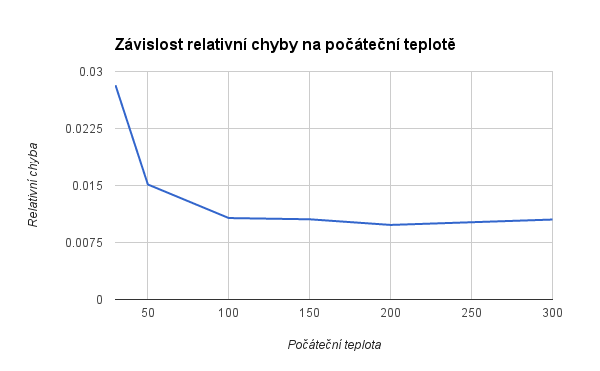
\includegraphics[width=0.99\textwidth]{1}
\end{figure}

\begin{figure}[H]\centering
 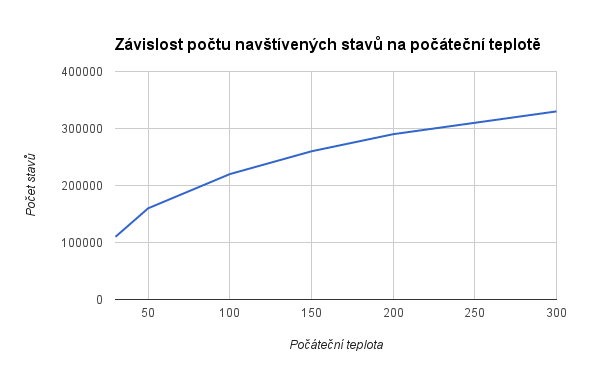
\includegraphics[width=0.99\textwidth]{2}
\end{figure}

Na naměřených datech je vidět, že pro teploty větší jak 100 se již nezmenšuje relativní chyba, zatímco počet stavů stále narůstá. Proto při tomto nastavení parametrů není již výhodné zvyšovat počáteční teplotu.

\begin{table}[H]
\centering
  \begin{tabular}{ |c|c|c|}
  \hline
  Ochlazování & Relativní chyba & Počet stavů \\
  \hline
  0,80 & 0,0186 & 110000 \\
  0,83 & 0,0166 & 130000 \\
  0,86 & 0,0132 & 160000 \\ 
  0,90 & 0,0099 & 220000 \\
  0,93 & 0,0080 & 320000 \\
  0,96 & 0,0062 & 570000 \\    
  0,99 & 0,0020 & 2300000 \\  
  \hline
  \end{tabular}
  \caption{Závislost chyby heuristiky na poměru kapacity batohu k sumární váze}
\end{table}

\begin{figure}[H]\centering
 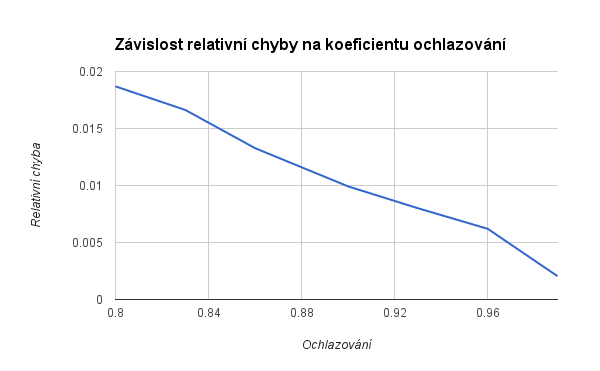
\includegraphics[width=0.99\textwidth]{3}
\end{figure}

\begin{figure}[H]\centering
 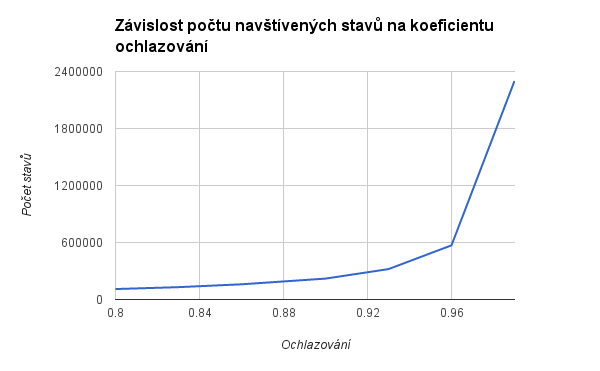
\includegraphics[width=0.99\textwidth]{4}
\end{figure}

Z grafů je možné vyčíst nejvýhodnější poměr chyby k počtu navštívených stavů a to u koeficientu ochlazování v rozmezí 0,92 -- 0,96.


\begin{table}[H]
\centering
  \begin{tabular}{ |c|c|c|}
  \hline
  Teplota tuhnutí & Relativní chyba & Počet stavů \\
  \hline
  80 & 0,0683 & 30000 \\
  50 & 0,0307 & 70000 \\
  30 & 0,0196 & 120000 \\ 
  20 & 0,0156 & 160000 \\
  10 & 0,0108 & 220000 \\
  5  & 0,0106 & 290000 \\    
  1  & 0,0094 & 440000 \\     
  \hline
  \end{tabular}
  \caption{Závislost chyby heuristiky na poměru kapacity batohu k sumární váze}
\end{table}

\begin{figure}[H]\centering
 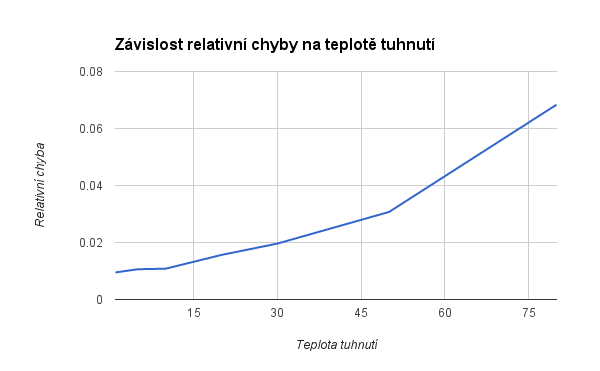
\includegraphics[width=0.99\textwidth]{5}
\end{figure}

\begin{figure}[H]\centering
 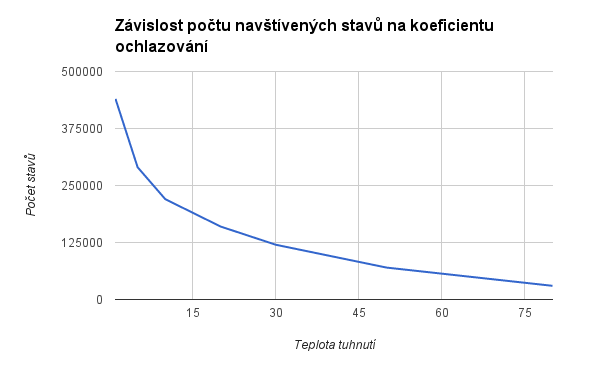
\includegraphics[width=0.99\textwidth]{6}
\end{figure}

Z naměřených dat se dá odhadovat ideální teplota tuhnutí okolo 20, kde vychází nejlépe poměr chyby k počtu navštívených stavů.

\begin{table}[H]
\centering
  \begin{tabular}{ |c|c|c|}
  \hline
  Equilibrium & Relativní chyba & Počet stavů \\
  \hline
  2  & 0,0201 & 88000 \\
  5  & 0,0132 & 220000 \\
  10 & 0,0065 & 440000 \\ 
  20 & 0,0043 & 880000 \\
  40 & 0,0020 & 1760000 \\
  80 & 0,0021 & 3520000 \\    
  \hline
  \end{tabular}
  \caption{Závislost chyby heuristiky na poměru kapacity batohu k sumární váze}
\end{table}

\begin{figure}[H]\centering
 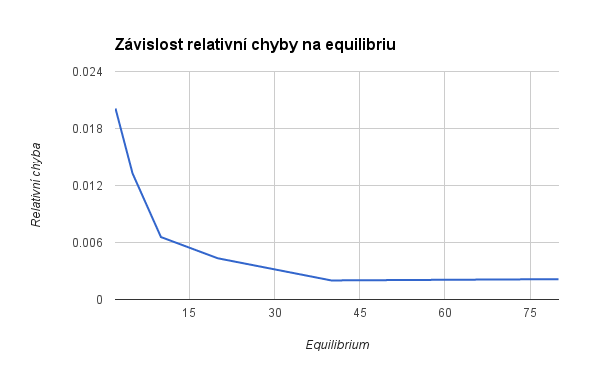
\includegraphics[width=0.99\textwidth]{7}
\end{figure}

\begin{figure}[H]\centering
 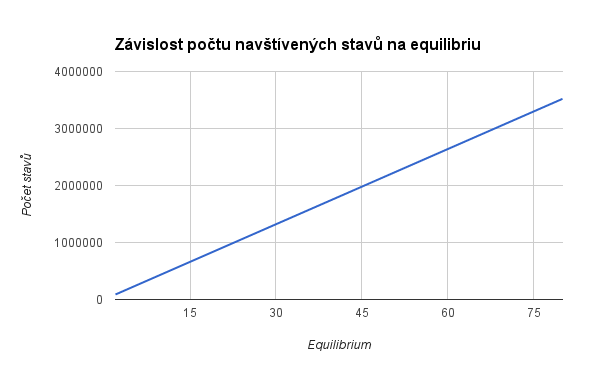
\includegraphics[width=0.99\textwidth]{8}
\end{figure}

Na grafech je viditelná lineární závislost počtu navštívených stavů na $equilibriu$. Protože je závislost chyby na $equilibriu$ spíše exponenciální klesající a od hodnoty $equilibrium = 40$ se relativní chyby téměř nemění, je usuzováno, že nejvýhodnější hodnota $equilibria$ je právě 40.

\section{Závěr}  
Algoritmus simulovaného ochlazování byl na implementaci jednoduchý, však na druhou stranu nastavování čtyřech parametrů bylo náročnější. To jsme navíc měli k dispozici exaktní řešení na výpočet relativní chyby. Bez těchto dat by bylo nastavování daleko obtížnější. Pokud bychom neměli k dispozici data pro výpočet relativní chyby, bylo by nutné spouštět algoritmus vícekrát a kontrolovat rozptyl nalezených řešení. Pokud by tento rozptyl byl malý, dala by se očekávat malá chyba vůči exaktnímu řešení.

U parametrů jako počáteční teplota a $equilibrium$ je nutné si dávat pozor, že při větších hodnotách již nedochází ke zlepšení výsledku, ale výpočetní náročnost stále roste. Následně také u koeficientu ochlazování od určitého bodu dochází k prudkému nárůstu navštívených stavů, zatímco chyba klesá stále téměř lineárně.

Metoda simulovaného ochlazování je na problém batohu použitelná. Při dobrém nastavení parametrů se dá dosáhnout rozumného poměru relativní chyby k výpočetní náročnosti.

\end{document}